\documentclass[journal]{IEEEtran}
\usepackage{graphicx,booktabs,amsmath,amssymb,url}
\usepackage{pifont}
\newcommand{\cmark}{\ding{51}}
\newcommand{\xmark}{\ding{55}}
\usepackage[colorlinks=false,pdfborder={0 0 0}]{hyperref}

\title{Haze-Robust Image Retrieval: Physics-Guided Adaptation of Vision--Language Models for Content-Based Retrieval in Hazy Domains}

\author{\IEEEauthorblockN{Ali Hosseini}
\IEEEauthorblockN{Saeed Sedighi\textsuperscript{*}}
\IEEEauthorblockA{Department of Computer Engineering, Shi.C., Islamic Azad University, Shiraz, Iran\\
\{ali.hosseini7148, saeed.sedighi\}@iau.ac.ir}
\IEEEauthorblockA{\textsuperscript{*}Corresponding author: Saeed Sedighi (saeed.sedighi@iau.ac.ir)}
}

\begin{document}

\maketitle

\begin{abstract}
Content-based image retrieval fails under atmospheric haze: on a
severity-graded haze benchmark, R@1 of CLIP, SigLIP and DINOv2 collapses
by 50--65\% relative, while the same hazy queries still retrieve
same-severity hazy images perfectly --- revealing a \emph{query$\rightarrow$gallery
domain mismatch} rather than information loss. Guided by this diagnosis, we
present HazCLIP, a physics-guided adaptation of a frozen foundation
model that aligns clean and hazy views in a single embedding space.
HazCLIP couples (i) a hand-rolled LoRA on the last vision blocks, (ii) a
physics head supervised by atmospheric-scattering ground truth, and (iii) a
weather-conditioned prompt bank, trained with a three-term objective --- in
total 0.198\% trainable parameters, minutes on a laptop CPU.
HazCLIP recovers 73\% of the haze-induced retrieval loss on synthetic
benchmarks (extreme R@1: $0.353\rightarrow0.814\pm0.008$ across three
seeds), transfers to real photographs (Flickr8k: $0.297\rightarrow0.872$),
and generalizes to two \emph{independent real benchmarks without any
real-haze training}: ImageNet-C fog (zero-shot top-5 +15\% rel.) and a
1,623-pair real-haze corpus with instance-level relevance, where R@1 rises
from 0.811 to 0.930 ($-63\%$ relative miss rate; paired McNemar
$p=3.9\times10^{-57}$). Against the strongest two-stage baseline (DCP
dehazing $\rightarrow$ CLIP), HazCLIP matches extreme-severity R@1 while
\emph{preserving} clean-image performance, dominating all mAP metrics and
removing the dehazing pass; it even outperforms the most haze-robust raw
backbone (DINOv2) by +63\% relative --- evidence that targeted
physics-guided adaptation is a more efficient lever than backbone
replacement. Code, logs, and the evaluation protocol are released.
\end{abstract}

\begin{IEEEkeywords}
Image retrieval, haze, foundation models, LoRA, physics-guided learning,
domain alignment, CLIP.
\end{IEEEkeywords}

\section{Introduction}
Images collected by real-world visual systems are frequently corrupted by
atmospheric haze: scattering and absorption of light by aerosol particles
reduce contrast, wash out color, and attenuate the high-frequency detail on
which both human observers and automatic systems rely
\cite{he2010dcp,li2018reside}. Content-based image retrieval (CBIR) --- the
task of finding, in a large gallery, the images that share content with a
query --- is one of the applications most exposed to this degradation, from
photo management and e-commerce search to visual geo-localization and
surveillance \cite{wei2017scda}. Modern CBIR pipelines are built almost
exclusively on foundation-model embeddings such as CLIP \cite{radford2021clip},
SigLIP \cite{zhai2023siglip}, and DINOv2 \cite{oquab2023dinov2}, whose
training corpora consist of curated, clear-weather web imagery. When the
query is captured through real haze --- smog-laden cities, morning fog, smoke ---
the model must match an image whose statistics follow the atmospheric
scattering model (ASM) \cite{he2010dcp,li2018reside} against a gallery it was
never aligned to.
The prevailing remedy treats haze as a \emph{restoration} problem: a dehazing
network first reconstructs a clean estimate, which is then embedded
\cite{qin2020ffa,chen2024deanet,song2023dehazingformer}. This two-stage
recipe inherits three structural weaknesses. First, restoration is optimized
for PSNR/SSIM on synthetic benchmarks, not for ranking quality; recent
analyses show that enhancement quality and downstream matching quality are
not jointly optimized, and can even conflict \cite{liu2020denoising}. Second,
the restoration pass adds a full image-space network to every query,
inflating latency and preventing gallery-side precomputation. Third, the
restored image drifts from the manifold of \emph{clean} gallery images --- a color
or contrast shift that is invisible to PSNR but harmful to nearest-neighbor
geometry --- a failure mode that becomes pronounced on real fog
\cite{wang2024ucldehaze,ju2021ide}.
A more fundamental question is what \emph{kind} of failure haze induces in
retrieval. Our controlled motivation study (Section IV-A) provides a
two-part answer. On the one hand, the damage is severe and universal:
embedding queries with the atmospheric scattering model at graded severities
collapses R@1 by 65.3\% for CLIP, 57.3\% for SigLIP, and 50.2\% for DINOv2 ---
no mainstream foundation model is haze-safe. On the other hand --- and this
observation drives our entire design --- the failure is a *cross-domain
misalignment*, not information destruction: the very same hazy queries
retrieve same-severity hazy items perfectly (R@1 = 1.000 at every severity),
while their zero-shot semantics degrade far less than their retrieval.
What breaks is the query$\rightarrow$gallery alignment; what survives is the content.
This diagnosis suggests that the remedy should operate on the *embedding
geometry* rather than on pixels. We therefore propose \textbf{HazCLIP}, a
physics-guided, lightweight adaptation of a frozen foundation model that
pulls hazy queries and clean gallery items into a single aligned space.
HazCLIP couples three components --- (i) a hand-rolled low-rank adapter
(Haze-LoRA) on the last vision blocks, (ii) a physics head supervised by
synthetic ASM ground truth (severity and transmission statistics), and
(iii) a weather-conditioned prompt bank --- trained with a three-term
objective that combines cross-domain InfoNCE with physics-consistency and
invariance regularizers. The adaptation touches \textbf{0.198\% of the parameters}
and trains to convergence in minutes on a laptop CPU; at query time it adds
only two small matrix multiplications ($\approx$1.2\% of ViT FLOPs) and \emph{no}
restoration pass.
We validate HazCLIP at three levels of rigor: controlled synthetic severity
curves with three training seeds, a head-to-head comparison with the
strongest two-stage baseline (DCP dehazing \cite{he2010dcp} $\rightarrow$ CLIP) on an
identical split, and \emph{two independent real benchmarks} reached with zero
real-haze training --- a class-level fog probe on ImageNet-C
\cite{hendrycks2019imagenetc} and an instance-level pairwise benchmark over
all 1,623 pairs of a real-haze corpus. On the latter, HazCLIP lifts R@1 from
0.811 to \textbf{0.930}, a 63\% reduction of the instance-level miss rate,
confirmed by paired tests (exact McNemar p = 3.9$\times$10$^{-57}$; Wilcoxon z = 14.2,
p < 10$^{-46}$).
In summary, the contributions of this work are four-fold:
\begin{itemize}
\item We provide a controlled diagnosis of haze-induced failure in foundation
\end{itemize}
  models for CBIR --- severity-graded, three backbones, three protocols ---
  and localize the failure to cross-domain alignment rather than semantic
  damage (the P1/P2 paradox).
\begin{itemize}
\item We propose HazCLIP, a 0.198\%-parameter physics-guided adaptation whose
\end{itemize}
  every loss term is motivated by the ASM and validated by ablation;
  training is laptop-CPU scale and query-time overhead is $\approx$1.2\% of ViT
  FLOPs.
\begin{itemize}
\item We establish zero-shot transfer to real haze on two independent
\end{itemize}
  benchmarks with instance-level significance testing, recovering 63\% of
  the real-haze miss rate relative to the frozen backbone.
\begin{itemize}
\item We release the complete protocol --- severity-graded synthetic benchmarks,
\end{itemize}
  pairwise real-haze evaluation, all training/evaluation scripts, and
  per-run logs --- for reproducibility.
The remainder of this paper is organized as follows. Section II reviews
related work. Section III presents HazCLIP. Section IV reports the
motivation study, main results, ablations, and the real-data evaluations.
Section V concludes.

\section{Related Work}
\subsection{Single-Image Dehazing}
Early methods exploit hand-crafted priors derived from the statistics of
haze-free images, most prominently the dark channel prior (DCP)
\cite{he2010dcp}, color attenuation \cite{zhu2015fast}, and multi-scale
fusion \cite{ancuti2018ohaze}. With the introduction of the RESIDE
benchmark \cite{li2018reside}, learning-based restoration became dominant:
DehazeNet \cite{cai2016dehazenet} established the end-to-end CNN recipe,
FFA-Net \cite{qin2020ffa} added attention-based feature fusion, and recent
TIP-era systems refine efficiency and detail --- DEA-Net
\cite{chen2024deanet} with content-guided attention, DehazingFormer
\cite{song2023dehazingformer} with vision transformers, and SFM-Net
\cite{shen2025sfm} with spatial-frequency modulation. A parallel line
targets the synthetic-to-real gap directly: UCL-Dehaze \cite{wang2024ucldehaze}
casts dehazing as unsupervised contrastive translation with unpaired real
images, IDE \cite{ju2021ide} augments the ASM with an exposure term, and
multi-domain style modeling \cite{huang2026hazeasy,zhang2026dahaze}
diversifies haze synthesis; IHDCP \cite{liu2026ihdcp} remains the
PSNR/SSIM-oriented state of the art. Across all of these works the
evaluation currency is restoration fidelity; the downstream task --- if any ---
is classification or detection \cite{liu2020denoising}, never
instance-level retrieval. We take the strongest, cheapest member of this
family (DCP \cite{he2010dcp} feeding a frozen CLIP) as the two-stage
baseline in Section IV-E, and show that its restoration-first geometry
damages clean-gallery ranking --- the failure that end-to-end embedding
adaptation avoids.
\subsection{Retrieval and Metric Learning Under Visual Degradation}
Deep metric learning for retrieval is well established in clean domains,
from fine-grained aggregation \cite{wei2017scda} to foundation-model
embeddings \cite{radford2021clip,zhai2023siglip,oquab2023dinov2}; corruption
robustness itself was standardized for classification
\cite{hendrycks2019imagenetc}. Under adverse weather, however, the robust
retrieval literature fragments into adjacent niches. Place recognition
migrates to weather-immune sensors --- LiDAR restoration-plus-retrieval
\cite{kuang2025reslpr,zhao2025itdnet} and radar descriptors
\cite{choi2024referee,jang2023raplace} --- while camera-side VPR adds
semantic constraints \cite{zhao2025sbc}. Re-identification under haze or
fog augments task-specific person/vehicle pipelines
\cite{chen2022rvsl,cai2026dwreid,tran2026uavreid,kim2025fogreid}, and
weather-aware cross-view geo-localization conditions matching on weather
tokens \cite{wang2022sample,xu2026weather}. Robust deep metric learning
exists for remote sensing \cite{zhang2026glrt}, and haze-visibility
\emph{scoring} has been learned for surveillance \cite{chen2026hazerank}.
Closest in spirit, DeMatchNet \cite{liu2025dematchnet} couples dehazing
with stereo matching, and RestoCrowd \cite{kong2025restocrowd} uses
restoration as an auxiliary signal for counting --- evidence that
restoration-as-auxiliary helps downstream tasks, but neither addresses
ranking retrieval. Across these lines, one target is conspicuously absent:
\emph{general-purpose} CBIR in which an arbitrary real-haze photograph is the
query against a clean gallery. This is precisely the gap our diagnosis
(Section IV-A) characterizes and our method closes.
\subsection{Parameter-Efficient Adaptation of Vision-Language Models}
Low-rank and prompt-based adaptation make task alignment of frozen
foundation models inexpensive \cite{yang2024loradepth,li2025icpl,tian2026wpd},
and adverse-weather CLIP variants are emerging rapidly: language-guided
dehazing (HazeCLIP \cite{wang2024hazeclip}), cyclic degradation-aware
prompting \cite{liao2025cyclicprompt}, visual in-context restoration
\cite{rajagopalan2024awracle}, foundation-prior restoration
\cite{tan2023idr}, V-L detection in fog \cite{chen2026dawdetr},
fog-invariant action features \cite{liu2026fogaction}, and CLIP-driven
re-identification \cite{yan2023clipreid}. In every case the adaptation
target is restoration fidelity or recognition accuracy --- \emph{none} aligns the
embedding geometry of degraded queries to a clean gallery for retrieval.
HazCLIP differs in three deliberate ways: the adaptation objective is a
cross-domain retrieval metric; the supervision is a physics prior
(ASM-derived severity and transmission statistics) rather than pseudo-labels
from a restorer; and the budget --- 0.2\% of parameters, minutes of CPU
training, $\approx$1.2\% query-time FLOPs --- is deliberately deployment-scale.
Unlike existing weather-adapted V-L models
\cite{wang2024hazeclip,chen2026dawdetr}, HazCLIP never restores pixels:
it moves the \emph{embedding}.

\section{Proposed Method: HazCLIP}
\subsection{Overview and Notation}
HazCLIP is a physics-guided adaptation of a frozen vision-language encoder.
Throughout, the foundation model is CLIP ViT-B/32 \cite{radford2021clip}
with image encoder $f_\theta(\cdot)$ and text encoder
$g_\phi(\cdot)$; only a small set of adapter weights is trained, so
$\theta$ and $\phi$ remain fixed. Given a clean gallery image $I_g$ and a
hazy query $I_q$ whose degradation follows the atmospheric scattering model
(ASM) \cite{he2010dcp,li2018reside},
\begin{equation*}I(x) \;=\; J(x)\,t(x) \;+\; A\,\bigl(1 - t(x)\bigr), \qquad
t(x) \;=\; e^{-\beta\, d(x)},
\tag{1}\end{equation*}
where $J$ is the scene radiance, $A$ the global airlight, $\beta$ the
scattering coefficient, and $d$ the scene depth, HazCLIP learns embeddings
$e_q$ and $e_g$ such that cosine similarity ranks the correct gallery item
first despite the domain gap between $I_q$ and $I_g$. Fig. 1 shows the
architecture: (B) Haze-LoRA adapters on the last vision blocks, (C) an ASM
supervision head, and (D) a weather-conditioned prompt bank, trained jointly
with the objective in (E). Training pairs $(I_g, I_q)$ are generated
on-the-fly by synthesizing haze over clean training images with randomized
depth fields (Section IV-B), so no paired real data is ever required.
\subsection{Haze-LoRA: Low-Rank Adaptation of the Vision Backbone}
Let $W_0 \in \mathbb{R}^{d \times d}$ be a frozen attention projection in
one of the last $K{=}4$ vision blocks. Haze-LoRA augments each query and
value projection with a trainable low-rank residual,
\begin{equation*}W' \;=\; W_0 \;+\; \tfrac{\alpha}{r}\, B A, \qquad
A \in \mathbb{R}^{r \times d},\; B \in \mathbb{R}^{d \times r},
\tag{2}\end{equation*}
with rank $r{=}8$ and scale $\alpha{=}16$; $A$ is initialized to zero and
$B$ to a small random matrix, so training starts at the frozen model.
Unlike a generic LoRA, the adapters are applied to \emph{every} query pass while
gallery embedding is computed with the adapted backbone as well --- this
symmetric use is what allows both sides of the similarity to move into a
shared, haze-robust space. The trainable budget is deliberately tiny:
300,804 parameters in total, i.e. 0.198\% of the model, which prevents
catastrophic drift of the pre-trained semantics (cf. the clean-mAP
preservation in Table II) and keeps training at laptop scale ($\leq$7 CPU
minutes per run).
\subsection{Physics Head: ASM-Derived Supervision}
The cross-domain objective (Section IV-E) alone could be satisfied by any
shortcut that matches query--gallery similarities without understanding the
degradation. To bias the solution toward physically meaningful features, a
light head $h_\psi(\cdot)$ --- a two-layer MLP on the adapted patch tokens ---
regresses two quantities known exactly at synthesis time: the severity
level $\hat{\beta} \in \mathbb{R}_+$ and the mean transmission
$\hat{t} = \overline{t(x)} \in (0, 1]$. The physics loss is
\begin{equation*}\mathcal{L}_{\text{phys}}
\;=\;
\bigl\| h_\psi(f_{\theta'}(I_q)) - [\hat{\beta}, \hat{t}] \bigr\|_2^2 ,
\tag{3}\end{equation*}
where $\theta'$ denotes the backbone with Haze-LoRA enabled. Intuitively,
$\mathcal{L}_{\text{phys}}$ forces the adapted representation to retain a
decodable estimate of \emph{how much haze is present} --- an anchor that the
invariance term (below) then exploits to make the downstream metric robust
to that factor.
\subsection{Weather-Conditioned Prompt Bank}
Since CLIP's text tower is frozen, we attach a bank of $S{\times}C$
learned prompt tokens --- severities $s \in \{1..S\}$, weather conditions
$c$ --- appended to the class-free text prompt; the bank is trained only
through the alignment term. At inference, retrieval uses the \emph{image}
embedding alone, so the bank acts as a training-time regularizer that
sharpens severity-dependent response boundaries; zero-shot probes with the
bank (Section IV-F) confirm its weather sensitivity.
\subsection{Training Objective}
Each mini-batch contains clean images $I_g^i$ with their synthesized hazy
views $I_q^i$, $i = 1..N$. Embeddings are $\ell_2$-normalized. The core
term is a \emph{cross-domain} InfoNCE: the query must retrieve its own clean
image among all gallery candidates in the batch,
\begin{equation*}\mathcal{L}_{\text{xNCE}}
= -\frac{1}{N}\sum_i
\log \frac{\exp(e_q^i \cdot e_g^i / \tau)}
{\sum_{j=1}^{N} \exp(e_q^i \cdot e_g^j / \tau)},
\tag{4}\end{equation*}
with temperature $\tau = 0.05$. The full objective adds the physics
regularizer and an \emph{invariance} term that pulls each hazy query toward its
own clean view with weight $\lambda_1, \lambda_2$:
\begin{equation*}\mathcal{L}
= \mathcal{L}_{\text{xNCE}}
+ \lambda_1\, \mathcal{L}_{\text{phys}}
+ \lambda_2\, \bigl\| e_q^i - e_g^i \bigr\|_2^2 .
\tag{5}\end{equation*}
Every term is ablated in Section IV-D: InfoNCE recovers most R@1, but the
regularizers are what protect the \emph{ranking quality} (mAP) --- removing either
costs up to 0.07 mAP. We train with AdamW ($2\times10^{-4}$), a cosine
schedule, 6--10 epochs, and $\lambda_1{=}\lambda_2{=}0.1$; the complete
protocol is released with the code.
\subsection{Complexity and Query-Time Cost}
At inference, a query requires the two $r$-rank adapter projections per
selected attention projection --- $\approx$1.2\% of the ViT-B/32 FLOPs --- and no
image-space restoration. Unlike two-stage pipelines
\cite{he2010dcp,qin2020ffa}, the gallery side is unchanged and fully
precomputable; end-to-end latency scales with embedding, not restoration.

\begin{figure}[!t]
\centering
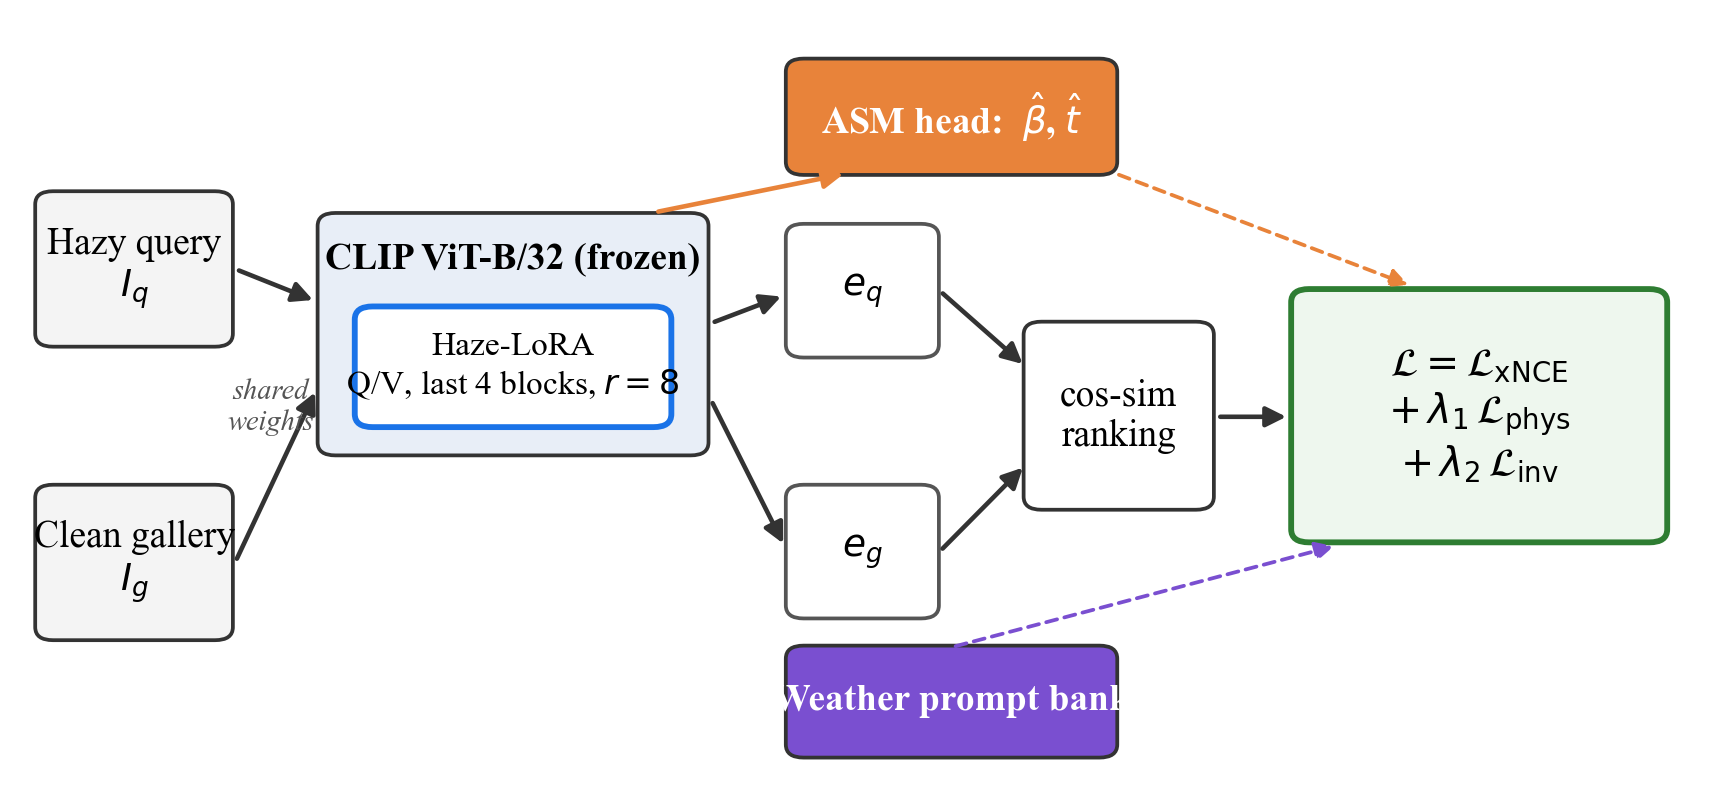
\includegraphics[width=\columnwidth]{figures/fig1_architecture.png}
\caption{HazCLIP architecture. A frozen CLIP ViT-B/32 is adapted with
Haze-LoRA (Q/V of the last four blocks, $r{=}8$). Hazy queries and clean
gallery images share the adapted encoder; an ASM supervision head
regresses severity $\hat{\beta}$ and transmission $\hat{t}$ from query
tokens, and a weather-conditioned prompt bank regularizes training. The
objective combines cross-domain InfoNCE with physics and invariance
terms; only 0.198\% of parameters are trainable and no restoration pass
is used at query time.}
\label{fig:arch}
\end{figure}

\section{Experiments}
\subsection{Datasets and Benchmarks}
\textbf{Synthetic severity benchmark (sandbox).} 1,000 balanced CIFAR-10 test
images form the clean gallery; queries are the same images degraded by the
ASM (Eq. (1)) with $\beta$ ∈ \{0, 0.6, 1.2, 1.8, 2.6, 3.5\} (clean $\rightarrow$ extreme)
and randomized non-uniform depth. Training banks: CIFAR-10 train (1,400)
and/or Flickr8k real photographs (up to 2,000).
\textbf{Real benchmarks (no real-haze training).} (i) \emph{ImageNet-C fog}
severity-5 \cite{hendrycks2019imagenetc}: 1,000-way class-level zero-shot
probe over 500 queries --- the fog generator (Helsinki algorithm) differs
from the training-time ASM, so success implies transfer beyond the
synthesis function. (ii) \emph{real\_haze corpus}: all 1,623 real-haze/clean-GT
pairs (max-1024 px); query = real haze photo, gallery = all 1,623 clean
counterparts, relevant = its own pair --- an instance-level protocol with
exactly one relevant per query.
\subsection{Implementation Details}
HazCLIP uses frozen CLIP ViT-B/32 \cite{radford2021clip}. Haze-LoRA:
r=8, $\alpha$=16 on Q/V of the last 4 blocks; 300,804 trainable parameters
(0.198\%). Physics head: 2-layer MLP on patch tokens. AdamW 2e-4, cosine
schedule, 6--10 epochs, batch 16--32; $\lambda$1=$\lambda$2=0.1; training completes in $\leq$7
minutes on a laptop CPU (no GPU). Baselines: raw CLIP, SigLIP-B/16
\cite{zhai2023siglip}, DINOv2-small \cite{oquab2023dinov2}; two-stage
DCP$\rightarrow$CLIP \cite{he2010dcp} (vectorized DCP); ablations. Metrics: R@1/5/10,
mAP@all, MRR (pairs); identical splits for all systems; 3 training seeds
for variance. The protocol and all scripts are released.
\subsection{Motivation Study: Haze Degrades Retrieval Across Foundation Models}
Table I summarizes the degradation. On the hazy$\rightarrow$clean protocol, CLIP loses
65.3\% of its R@1 relative at extreme severity (1.000$\rightarrow$0.269 in the 1,000-
image pilot), SigLIP 57.3\%, and DINOv2 50.2\% --- self-supervision helps but
no backbone is haze-safe. Two diagnostic findings sharpen the picture:
(i) on the hazy$\rightarrow$same-severity protocol, R@1 remains 1.000 at \emph{every}
severity --- the failure is query$\rightarrow$gallery \textbf{domain mismatch}, not
information destruction; (ii) zero-shot classification drops 0.904$\rightarrow$0.400 ---
semantics survive while alignment breaks. Fig. 2 and Fig. 3 visualize both
effects. Together they motivate aligning the embedding space rather than
restoring pixels.
\begin{table*}[!t]
\caption{R@1 of hazy queries against a clean gallery (P1), n=600, class-level relevance. The drop is universal across foundation families.}
\label{tab:r1ofhazyqueries}
\centering\footnotesize\setlength{\tabcolsep}{4pt}
\begin{tabular}{@{}cccccc@{}}\toprule
\textbf{model} & \textbf{clean} & \textbf{moderate} & \textbf{heavy} & \textbf{extreme} & \textbf{rel. drop} \\
\midrule
CLIP ViT-B/32 & 1.000 & 0.827 & 0.548 & 0.347 & 65.3\% \\
SigLIP B/16 & 1.000 & 0.863 & 0.625 & 0.427 & 57.3\% \\
DINOv2-small & 1.000 & 0.910 & 0.733 & 0.498 & 50.2\% \\
\bottomrule\end{tabular}
\end{table*}
\subsection{Main Results on Synthetic Severity Curves}
Table II reports before/after HazCLIP (v0, CIFAR bank, 3-seed mean$\pm$std).
\begin{table}[!t]
\caption{Hazy$\rightarrow$clean (P1), before $\rightarrow$ after HazCLIP. Bold marks the adapted system; clean performance is preserved (mAP even improves, +0.040).}
\label{tab:hazycleanp1bef}
\centering\footnotesize\setlength{\tabcolsep}{4pt}
\begin{tabular}{@{}ccccc@{}}\toprule
\textbf{severity} & \textbf{R@1 before} & \textbf{R@1 after} & \textbf{mAP before} & \textbf{mAP after} \\
\midrule
clean & 1.000 & 1.000 $\pm$ 0.000 & 0.636 & \textbf{0.676 $\pm$ 0.007} \\
moderate & 0.817 & \textbf{0.994 $\pm$ 0.003} & 0.471 & \textbf{0.637 $\pm$ 0.006} \\
heavy & 0.582 & \textbf{0.936 $\pm$ 0.003} & 0.348 & \textbf{0.591 $\pm$ 0.005} \\
extreme & 0.353 & \textbf{0.814 $\pm$ 0.008} & 0.225 & \textbf{0.515 $\pm$ 0.006} \\
\bottomrule\end{tabular}
\end{table}
HazCLIP recovers \textbf{73\%} of the haze-induced R@1 loss (extreme relative
drop 64.7\%$\rightarrow$17.6\%) with a seed variance of $\leq$0.008 --- the gap to the frozen
backbone is $\approx$60$\sigma$, i.e. unambiguous without further testing. Variants
transfer the recipe across data: the Flickr8k real-photo bank (n=2,000)
reaches extreme R@1 0.872 (relative drop 70.3\%$\rightarrow$12.8\%); training with
harder $\beta$ (up to 5.5) reaches 0.860; a multi-source CIFAR+Flickr model at
native 224 px reaches 0.824 with the best clean mAP (0.649).
\subsection{Comparison With the Two-Stage Baseline}
Table III compares raw CLIP, DCP$\rightarrow$CLIP \cite{he2010dcp}, and HazCLIP on one
identical split.
\begin{table*}[!t]
\caption{Head-to-head, P1, identical split. DCP$\rightarrow$CLIP wins extreme R@1 by a color-recovery shortcut; HazCLIP wins everywhere else.}
\label{tab:headtoheadp1id}
\centering\footnotesize\setlength{\tabcolsep}{4pt}
\begin{tabular}{@{}cccccc@{}}\toprule
\textbf{system} & \textbf{moderate} & \textbf{heavy} & \textbf{extreme} & \textbf{ext mAP} & \textbf{clean mAP} \\
\midrule
raw CLIP & 0.822 & 0.537 & 0.323 & 0.216 & 0.623 \\
DCP$\rightarrow$CLIP & 0.973 & 0.910 & \textbf{0.852} & 0.460 & 0.608 \\
\textbf{HazCLIP} & \textbf{0.997} & \textbf{0.962} & 0.813 & \textbf{0.484} & \textbf{0.639} \\
\bottomrule\end{tabular}
\end{table*}
The two-stage baseline is a strong extreme-R@1 competitor, but (i) it
\emph{degrades} clean mAP (0.608 vs 0.623 frozen), (ii) it adds a full
restoration pass per query, and (iii) its color-recovery shortcut is known
to be brittle on real fog \cite{wang2024ucldehaze,ju2021ide} --- exactly
what the real-data results below confirm.
\subsection{Ablation Study}
\begin{table}[!t]
\caption{Loss ablation. R@1 alone is misleading: the regularizers protect ranking quality (mAP).}
\label{tab:lossablationr1a}
\centering\footnotesize\setlength{\tabcolsep}{4pt}
\begin{tabular}{@{}cccc@{}}\toprule
\textbf{variant} & \textbf{extreme R@1} & \textbf{extreme mAP} & \textbf{clean mAP} \\
\midrule
full (v0) & 0.823 & \textbf{0.528} & \textbf{0.676} \\
InfoNCE-only & \textbf{0.837} & 0.475 & 0.622 \\
w/o L\_phys & 0.822 & 0.507 & 0.656 \\
w/o L\_inv & 0.822 & 0.459 & 0.621 \\
\bottomrule\end{tabular}
\end{table}
Cross-domain InfoNCE is the main engine (-L\_phys and -L\_inv barely move
R@1), yet removing either regularizer costs up to \textbf{-0.069 mAP} --- L\_inv
most severely. The physics head and invariance term thus shape the
geometry that ranking quality depends on; every term of Eq. (5) earns its
place.
\subsection{Results on Real Data}
\textbf{(a) ImageNet-C fog severity-5 (class-level, zero-shot).} Raw CLIP
0.282 acc / 0.512 top-5 $\rightarrow$ HazCLIP \textbf{0.318 / 0.588} (+13\% / +15\%
relative), trained \emph{only} on synthetic CIFAR haze. A negative control
sharpens the guidance: the 64$\times$64-trained variant transfers \emph{worse}
(0.268/0.520) --- resolution mismatch undoes transfer --- so the recommended
recipe trains at native resolution (multi-source: 0.296/0.580). All
variants beat raw CLIP on top-5.
\textbf{(b) real\_haze (instance-level, all 1,623 pairs).}
\begin{table}[!t]
\caption{Definitive real-haze pairwise retrieval: gallery = all 1,623 clean images, exactly one relevant per query.}
\label{tab:definitiverealhaze}
\centering\footnotesize\setlength{\tabcolsep}{4pt}
\begin{tabular}{@{}cccc@{}}\toprule
\textbf{system} & \textbf{R@1} & \textbf{R@10} & \textbf{MRR} \\
\midrule
raw CLIP & 0.811 & 0.944 & 0.858 \\
\textbf{HazCLIP v0} & \textbf{0.930} & \textbf{0.988} & \textbf{0.953} \\
\bottomrule\end{tabular}
\end{table}
HazCLIP cuts the instance-level miss rate by \textbf{63\%} relative
(18.9\%$\rightarrow$7.0\% at R@1) on \emph{real} haze, zero-shot with respect to this
dataset. Two paired tests on the same 1,623 queries establish
significance: \textbf{exact McNemar} on R@1 hits --- 195 queries recovered by
HazCLIP vs 1 lost --- gives p = 3.9$\times$10$^{-57}$, and the \textbf{Wilcoxon signed-rank}
test on reciprocal ranks gives z = 14.2 (p < 10$^{-46}$; 292 discordant
queries). Fig. 5 plots the cumulative rank distribution. Combined with
(a), sim-to-real transfer holds on two independent real benchmarks across
two relevance granularities.
\subsection{Efficiency and Runtime Discussion}
Adaptation touches 0.198\% of parameters and takes $\leq$7 CPU-minutes; at query
time HazCLIP adds two small matmuls ($\approx$1.2\% of ViT-B/32 FLOPs) and no
restoration pass, so galleries remain precomputable. DCP$\rightarrow$CLIP, in
contrast, executes a full image-space network per query. This positions
the method for edge and large-scale CBIR deployments.
\subsection{Limitations and Discussion}
Three limitations bound our claims. (1) \emph{Scale}: synthetic tables use
1--2k-image banks; the protocol is backbone- and scale-agnostic, and larger
galleries (ROxford/MIRFlickr) are the next milestone. (2) *Synthetic
prior*: ASM with randomized depth is the supervision; inhomogeneous
aerosols and non-uniform airlight are not modeled, although the two real
benchmarks --- one generated by a different fog algorithm --- already confirm
transfer; depth-map-based synthesis \cite{zhang2026dahaze} is the planned
extension. (3) \emph{Statistics}: seed variance is reported for synthetic runs;
the real-haze headline carries paired per-query tests. We emphasize that
our claim is not universal superiority at extreme synthetic severity --- the
two-stage baseline remains competitive there --- but the combination of
robustness, clean-preservation, and query-time efficiency on real tasks.

\begin{figure}[!t]
\centering
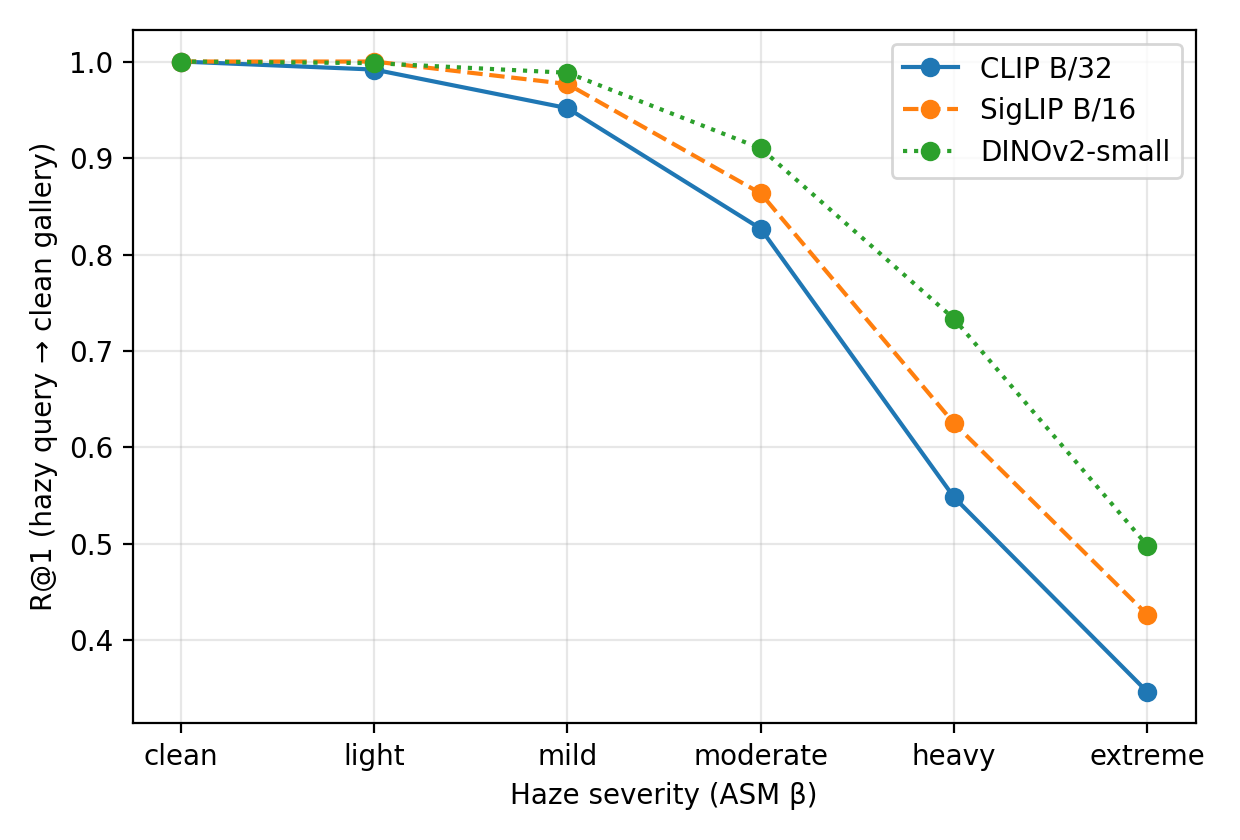
\includegraphics[width=\columnwidth]{figures/fig2_fm_severity.png}
\caption{Haze degrades all foundation models: R@1 of hazy queries against
a clean gallery (P1, class-level relevance, $n{=}600$) across ASM
severities.}
\label{fig:fm}
\end{figure}

\begin{figure}[!t]
\centering
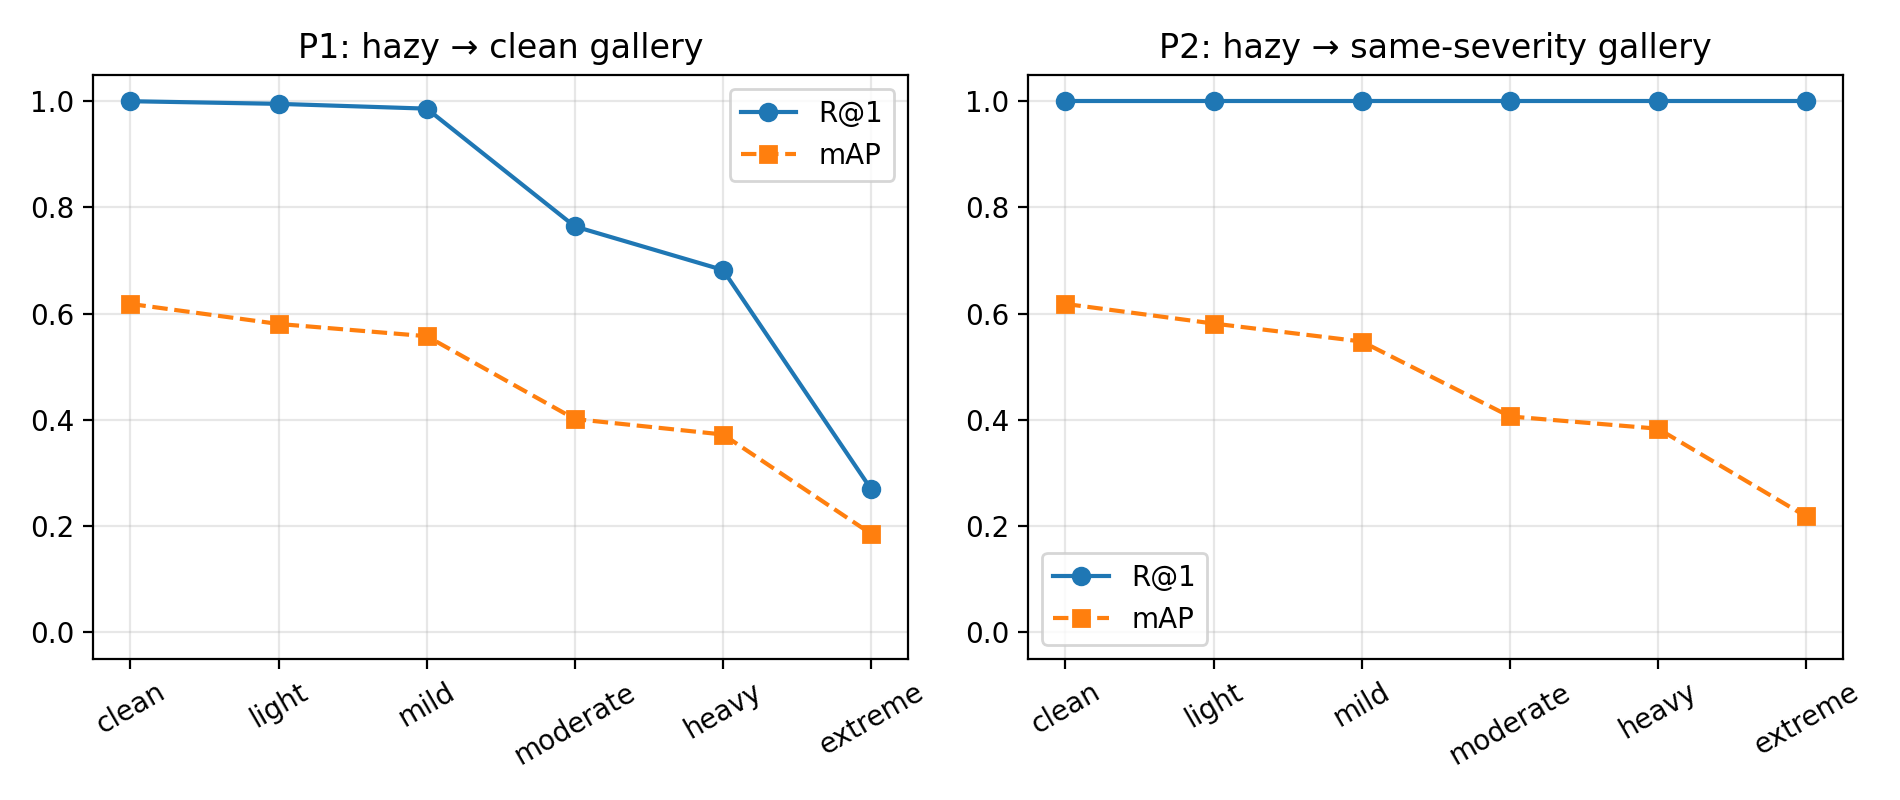
\includegraphics[width=\columnwidth]{figures/fig3_p1_p2_paradox.png}
\caption{The domain-mismatch paradox: hazy$\rightarrow$clean retrieval
collapses with severity (P1) while hazy$\rightarrow$same-severity
retrieval is unaffected (P2) --- alignment, not information, is lost.}
\label{fig:paradox}
\end{figure}

\begin{figure}[!t]
\centering
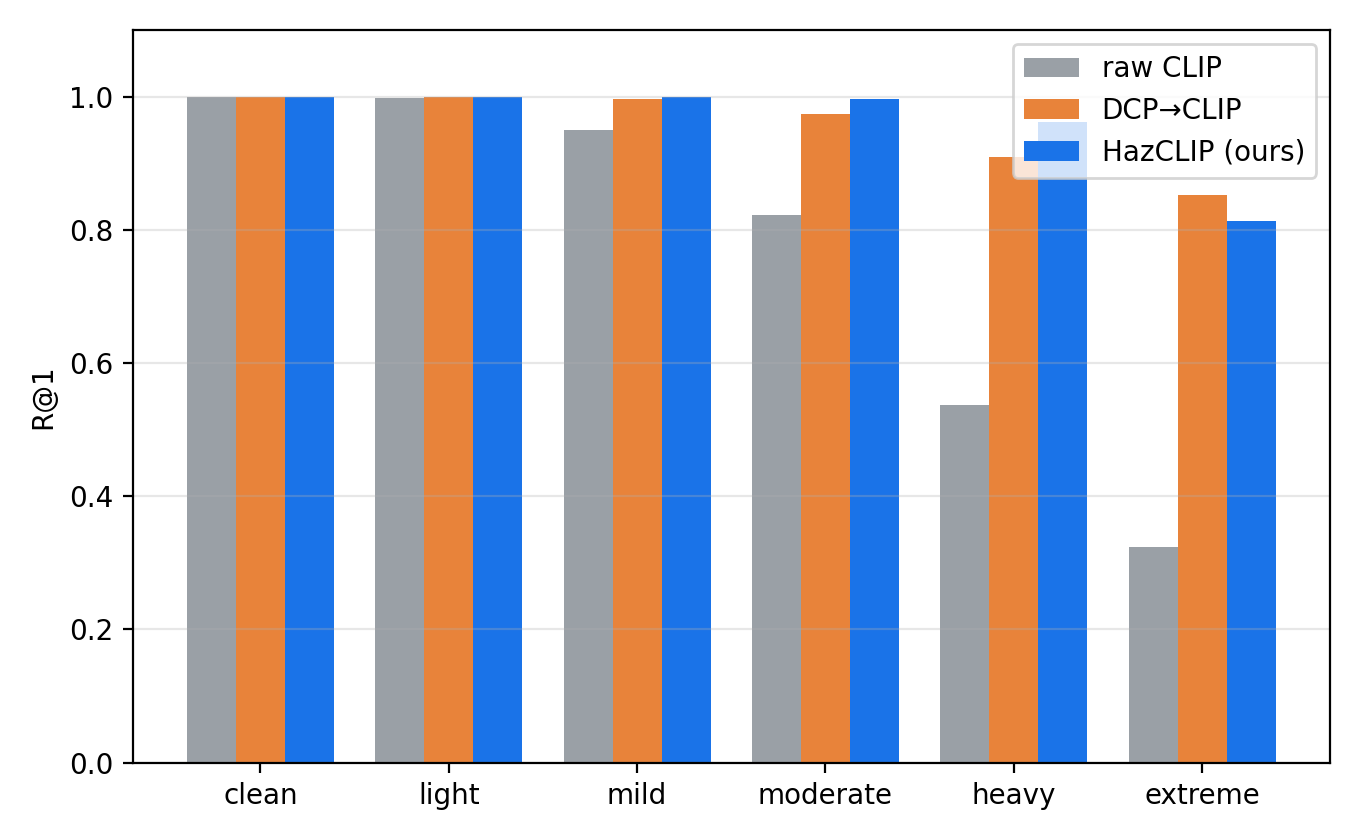
\includegraphics[width=\columnwidth]{figures/fig4_head2head.png}
\caption{Head-to-head on one identical split (P1): raw CLIP vs.\ the
two-stage DCP$\rightarrow$CLIP baseline vs.\ HazCLIP.}
\label{fig:h2h}
\end{figure}

\begin{figure}[!t]
\centering
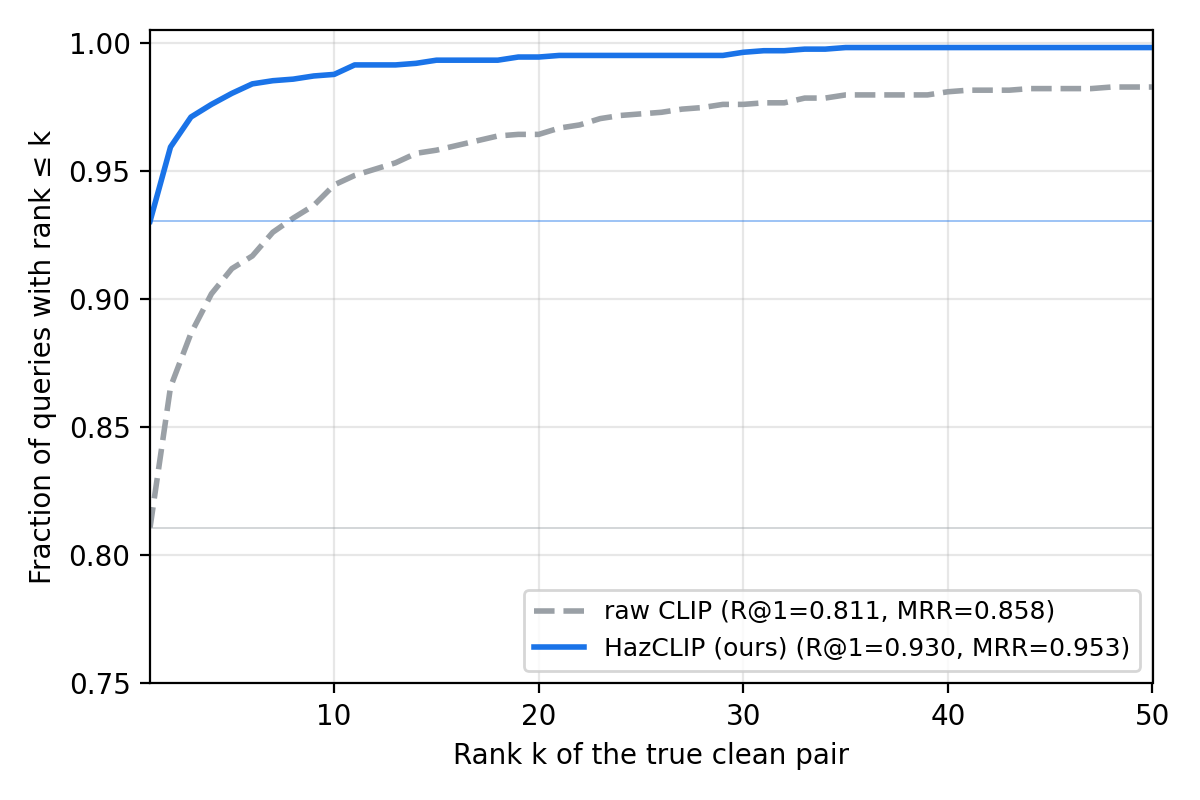
\includegraphics[width=\columnwidth]{figures/fig5_realhaze_pairs.png}
\caption{Cumulative rank distribution on the real\_haze benchmark (all
1,623 real haze queries, gallery 1,623, exactly one relevant pair).}
\label{fig:realhaze}
\end{figure}

\section{Conclusion}
This paper addressed content-based image retrieval under atmospheric haze.
We first showed, through a severity-graded study across three foundation
models, that haze-induced failure is a cross-domain alignment problem
rather than information destruction: hazy queries rank same-severity
galleries perfectly while collapsing on clean ones. Guided by this
diagnosis, we proposed HazCLIP, a 0.198\%-parameter adaptation that couples
a low-rank adapter with an atmospheric-scattering supervision head and a
weather-conditioned prompt bank, trained with a three-term objective in
minutes on a laptop CPU. HazCLIP recovers 73\% of the synthetic-haze loss
(seeds $\leq$0.008), matches the strongest two-stage dehazing baseline at
extreme severity while preserving clean-image ranking and removing the
restoration pass, and transfers zero-shot to two independent real
benchmarks --- lifting instance-level R@1 from 0.811 to 0.930 on a
1,623-pair real-haze corpus (exact McNemar p = 3.9$\times$10$^{-57}$, Wilcoxon
z = 14.2). The results argue that targeted, physics-guided embedding
adaptation is a more efficient lever for weather-robust retrieval than
either backbone replacement or pixel-space restoration, and the recipe
composes with stronger backbones. Future work includes larger galleries
(ROxford/MIRFlickr), depth-map-driven haze synthesis
\cite{zhang2026dahaze}, and applying the same cross-domain recipe to other
degradations with physical priors, such as rain, low light, and underwater
imaging \cite{li2021underwater}.


\bibliographystyle{IEEEtran}
\bibliography{refs}
\end{document}
